\chapter{Background} \label{chap:back}
%\section*{} \label{sec:...}
%\begin{dummied}
%\end{dummied}
\section{Problem Statement} \label{sec:cul_problem}
    It's typical for researchers to have a forward-looking aptitude towards their work, and to come up with ideal realities that they wish or find inevitable that will be found fleshed out. This is how in 1991, Mark Weiser described the concept of Ubiquitous Computing\cite{ weiser1991}, a concept that is today taken for granted in the dawn of IoT computing, taking only as a basis the observable trend of miniaturization of electronic components and wireless communication. As such, it’s not hard to imagine that the path ahead for Human-Computer Interaction has been broadly discussed, as well as its concerns and criticisms. Gestural Detection technology may appear like a modern innovation of the last decade, but it was sought after for several before, and it took progressive iteration, evolution, to reach this state.\\
    However not all evolutions in a field are continuous, there are points in a macroscopic view of technology where discrete advancements have to be made. This describes the paradigm shifts encountered in the major approaches to HCI. Just like he Graphical User Interface (GUI) came to outperform the Command Line Interface (CLI) in several use cases, now the once predicted Natural User Interface (NUI) shows potentials to outperform the GUI in select applications.\\
    However, just how the initial GUI’s were rudimentary, and faced design constraints that were ironed out with the growth of the supporting hardware and with the emergence of technological literacy, so does now the NUI have its own problems. As was further described in the introductory chapter \ref{sec:intro_motivation}, the NUI as a concept for Gestural Interfaces is not realized, still has room for cultivation, and the Shamanic Interface proposal intends to contribute through an holistic vision of human communication and computer interaction as a whole.

\section{Shamanic Interface} \label{sec:cul_shaman}
    The Shamanic Interface takes its inspiration from the science fiction book Freedom, by Daniel Suarez, from which the name is directly lifted. In the fictional plot, the Shamanic Interface is a mechanism by which the characters apply commands to a complex augmented reality system, through use of somatic gestures.\\
    
    \emph{“It’s called the shamanic interface because it was designed to be comprehensible to all people on earth, regardless of technological level or cultural background”}\\
    
    The argument suggested by the book was the universality of beliefs in immaterial concepts, and how they may be accessed and communicated through ceremonial and traditional gestures. The futuristic technology described leveraged these rituals, gesticulations, and made it its own form of input, connecting its user experience to acts that almost appear as if magical, where the virtual environments reacts and materializes in accordance to motion in a way that gives a logical and natural impression to anyone. However, while gesticulations and emblematic motion are indeed common to human behaviour, the notion that a single set of gestures that could be understood by all people of the world exists is unfounded and too fantastic for real practical implementation, as seen later in this chapter, namely from the contradictions found within the meaning of same gestures across cultures. For this reason, when Morgado\cite{MOR2013} contemplated the solution taking the fantastical interface as a basis, the name “anti-shamanic” was also pondered upon as his proposal subverts and deviates from this conception.\\
    The valuable aspect of focus was the engineering of a system that adapts to the immanent semantics as a form of command for virtual environments. To achieve this, the proposal of the Shamanic Interface required an addendum as such: To decouple the concerns of gestural identification and parameterization, and those of command classification and execution, potentially through distinct software layers. Thus, enabling customized mapping of different collections of cultural gestures onto commands. The ensuing result is that commands in the application layer of a system are independent from the actual motion of the user, and it can conversely make a choice of mappings that best fit the needs and requirements of the user.\\ 
    In other words, a real Shamanic Interface would be an adaptable system with a customized experience, that allows users to establish links between their learned communal meanings and the application’s commands. This is how it is expected for it to tackle the current limitations found in NUIs, where performing those commands usually adopts a mimicry approach. It is expectable that this way, the SI will allow the NUIs to overcome the difficulties of exploration and learning attached to the method. Other problems that this may directly favour NUIs with are the issues of accessibility for users with physical impairments and handicaps who are incapable of performing the current required gestures, such as wheelchair-bound users, and allowing interaction to appear visibly more natural for external observers, thus making usage of this systems more societally acceptable.\\ 
    Prior work was performed on Shamanic Interfaces\cite{pinto2015}, including a research paper where a research tool was developed for testing and expanding on the concept of Shamanic Interfaces. The developed application was in a working condition, capable of identifying cultural gestures, however it specifies performing the actual tests as a requirement among future work. In this work we look to give continuity to the development and use of that tool.


\section{Culture in HCI} \label{sec:cul_HCI}
    Culture is a notoriously difficult term to define. In a more general sense, culture is interpreted in the aspects of a society’s artistic productions, their traditions, the system of beliefs held by the populous and their modes of expression. Usually driven by symbols which have values attached, which themselves are regarded thanks to attitude or faith of the community in those values. However the interest in culture is restrained to, from one view in HCI as described by Hofstede\cite{hofstede1986}, the \emph{“collective programming of the mind which distinguishes the members of one human group from another”}. The distinctions between cultures, leads to different approaches to communication, learning, admissibility and work ethic, which in turn, signifies differences in how people will interact with other people, and with technology.\\
    Cultural diversity is a challenge for HCI. The widespread adoption of the GUI is one aspect of what is considered the apparent process of globalization. Businesses outgrow their national boundaries, form a global presence and ship products even to developing countries. Technology itself promotes international growth thanks to the existence of the world wide web, social media, new forms of communication, advertisement and even vectors for outsourced manpower. As such, it’s not unusual to find products and services that break the cultural boundaries. This multi-culturalism often proves to be an obstacle towards the usability of the system\cite{mapp2004} leading to rejection or slow adoption within certain communities without additional differentiating work applied to it. In recent review works on the subject of culture and HCI, the distinction between visible and invisible attributes or indicators was made, with visible attributes relating to interface design and localization issue, while invisible attributes pertain to Hofstede’s theory of cultural dimensions\cite{hofstede1986}\cite{mintu1992cultures}. One example of dimension is the Power Distance, which levels how receptive users are to inequalities among other members of a society, a result of individualism\cite{erumban2006}. This would be relevant in the case of online gaming, where western audiences find the concept of paying for power unacceptable, but asian players state they find no issue with the practice.\\
    And as such, culture is a highly researched topic in HCI, as no singular approach will exist for an interface because of culture. And this is the obstacle of culturally-aware systems. It is expectable of them to adapt to the users’ needs in all stages of HCI design, which means, as opposed to creating different builds for each context, the systems must include cultural models as well as generate adaptation rules. From the visible indicators, these include the presentation of information, the language, the dialog design and the interaction design itself\cite{duncker2013}\cite{erumban2006}.\\ 
    Here, the shamanic interface may be pertinent to the latter, as it models and integrates socio-cultural information relevant to user background.\\



\section{Cultural Gestures} \label{sec:cul_Cultural_Gestures}
    One important task to prior to the development of the goals was to answer the question of what gestures are, and how does motion relate to meaning. We know that gestures play a role in communication and learning\cite{pine2004more}\cite{macedonia2012gestures}, but we seek out a definition of gesture that would provide an understanding of the information by them encoded. The field of gestural study covers this as well as other topics\cite{kendon1996agenda}, such as their kinetics and shape, however, the typology of consequence, is the relationship between gesture and verbalizations. Gestures can be produced in conjunction with speech, in alternation or replacement of speech, or as their own utterances. \\
    Gestures had prior classifications but were categorized, based past work in the field, in a singular set by Adam Kendom\cite{mcneill1987} along a continuum of closeness to speech or, opposite to that, to metaphorical allusion. Wherein, the following five types of gestures were distinguished and still today referenced\cite{mcneill2014}\cite{mitra2007}: \textbf{Gesticulations} are spontaneous movements that accompany speech. These consist of 90\% of the gestures performed by humans and are most usually started imperceptibly, often accompanying strokes in the semantic pattern of utterances, usually synchronizing or preceding emphasis and pauses. Their prevalence is universal in human nature, and not necessarily applicable as an act of communication, as the interlocutor in a phone conversation will often perform these gestures as an aid in speech production; \textbf{Speech-Framed Gestures} are gestures that are a part of the spoken sentences themselves. These replace words directly. They’re no co-expressive the same way gesticulations were, instead replacing a grammatical hole in the message; \textbf{Pantomimes} are used within a similar fashion, but these do not aid verbal communication. Epitomized with the description of “Dumb-show”, it’s any exaggerated mimicry that describes a shape, an action or any other physical concept. \textbf{Emblems} which are familiar symbology conventionalized within a specific culture, translating directly to a specific significance. The meanings are vastly diverse, ranging from polite, to less-than-so, such as they’re addressed informally as ‘quotable gestures’. Despite their innate substance, they can naturally be interweaved with one another or with speech itself as a form of gesticulation. Their meaning is powerful and long lived, such as that many emblems have outlasted their own historical roots, the languages that could describe their meanings they co-existed with. \textbf{Sign languages} which are fully fledge lexicons, with their own linguistic structures, including that of grammatical patterns and vocabulary. These do not directly correlate to that of a native language and have evolved out of the necessity of coordination with speech, with the practice of signing and speaking frequently proving to be a disruption for practitioners.\\
    Of these, the ones that most interest our work are the emblems. Culturally charged gestures with a basis on the background their users originate from, such as the thumbs up, or the tongue protrusion. While an accomplished shamanic interface wouldn’t restrict itself to simply detecting emblems, these have the strongest link between a natural movement and an inferred interpretation, and thus, are the most promising towards the primary contribution of the proposal. Also, on their own, they function as idioms, potentially having multiple denotations, and as thus, a rigid system would not be able to utilize one without facing eventual need of teaching them to the user, or directly clashing with the expectation of users from different contexts.\\
    In the past work \cite{pinto2015}, an example list of emblems was researched. The following table \ref{tab:Table_Emblems_Morris} is a summary of information that was sourced from David McNeill’s article\cite{mcneill1994} on gestures, however, the examples were also themselves further sourced to Desmond Morris’ findings on an earlier book\cite{morris1979} from which the accompanying figure \ref{fig:Figure_Emblems_Morris} is sourced. With the prospect of having a more complete set of gestural emblems as a basis for the requirements of the thesis’ work, a later dictionary-like publication by Morris featuring over three hundred gestures that could be contemplated as meaningful was obtained.


\begin{table}
    \centering
    \caption{\label{tab:Table_Emblems_Morris}20 examples of Emblems, their meaning and distribution}
    \begin{tabular}{|l|l|l|}
        \hline
        Sign Name       & Cultural Background   & Meaning   \\ \hline\hline
        \multirow{2}{*}{Fingertip Kiss} & Holland, Belgium, Yugoslavia and Turkey   & Praise\\ \cline{2-3} 
            & Portugal, Sardinia, Malta and Corfu   & Salutation    \\ \hline
        \multirow{2}{*}{FingerCross}    & England, Scandinavia, parts of Sicily, and Yugoslavia & Protection\\ \cline{2-3} 
            & Corfu and Turkey  & Breaking a friendship\\ \hline
            The Nose Thumb  & Everywhere    & Mockery\\ \hline
        \multirow{4}{*}{The Hand Purse} & Italy, Sardinia and Sicily    & Query\\ \cline{2-3} 
            & Portugal, Greece and Turkey   & Good\\ \cline{2-3} 
            & Belgium and France    & Fear\\ \cline{2-3} 
            & Holland and Germany   & Emphasis\\ \hline
        \multirow{2}{*}{Cheek Screw}    & Italy, Sicily and Sardinia    & Good to eat\\ \cline{2-3} 
            & Germany   & Crazy\\ \hline
        \multirow{2}{*}{Eyelid Pull}    & Italy & Watch out, be alert\\ \cline{2-3} 
            & Everywhere else   & I’m alert\\ \hline
        Forearm Jerk            & North America                                     & Italian Salute\\ \hline
        Flat-Hand Flick         & Belgium, France, Italy and Greece                 & Beat it\\ \hline
        \multirow{5}{*}{Ring}   &                                                   & OK\\ \cline{2-3} 
                                & Tunisia                                           & Threat\\ \cline{2-3} 
                                & Brazil                                            & Insult\\ \cline{2-3} 
                                & Germany, North Italy, Northern Sardinia and Malta & Orifice\\ \cline{2-3} 
                                & Belgium, France and Tunisia                       & Zero\\ \hline
        Vertical Horn                     & Spain, Portugal and Italy & Cuckold        \\ \hline
        Horizontal Horn                   & Malta and Italy           & Protection     \\ \hline
        \multirow{2}{*}{Fig}              &                           & Sexual comment \\ \cline{2-3} 
                                          &                           & Insult         \\ \hline
        \multirow{2}{*}{Head Toss}        &                           & Negation       \\ \cline{2-3} 
                                          &                           & Beckoning      \\ \hline
        \multirow{2}{*}{Chin Flick}       &                           & Disinterest    \\ \cline{2-3} 
                                          &                           & Negation       \\ \hline
        Cheek Stroke                      &                           & Thin and ill   \\ \hline
        Thumb Up                          &                           & OK             \\ \hline
        \multirow{2}{*}{Teeth-Flick}      &                           & Nothing        \\ \cline{2-3} 
                                          &                           & Anger          \\ \hline
        \multirow{2}{*}{Ear Touch}        &                           & Effeminate     \\ \cline{2-3} 
                                          &                           & Watch out      \\ \hline
        \multirow{2}{*}{Nose Tap}         &                           & Secrecy        \\ \cline{2-3} 
                                          &                           & Insult         \\ \hline
        \multirow{2}{*}{Palm-back V-sign} &                           & Victory        \\ \cline{2-3} 
                                          & Britain                   & Sexual insult  \\ \hline
                                        
    \end{tabular}
\end{table}

\begin{figure}
    \centering
    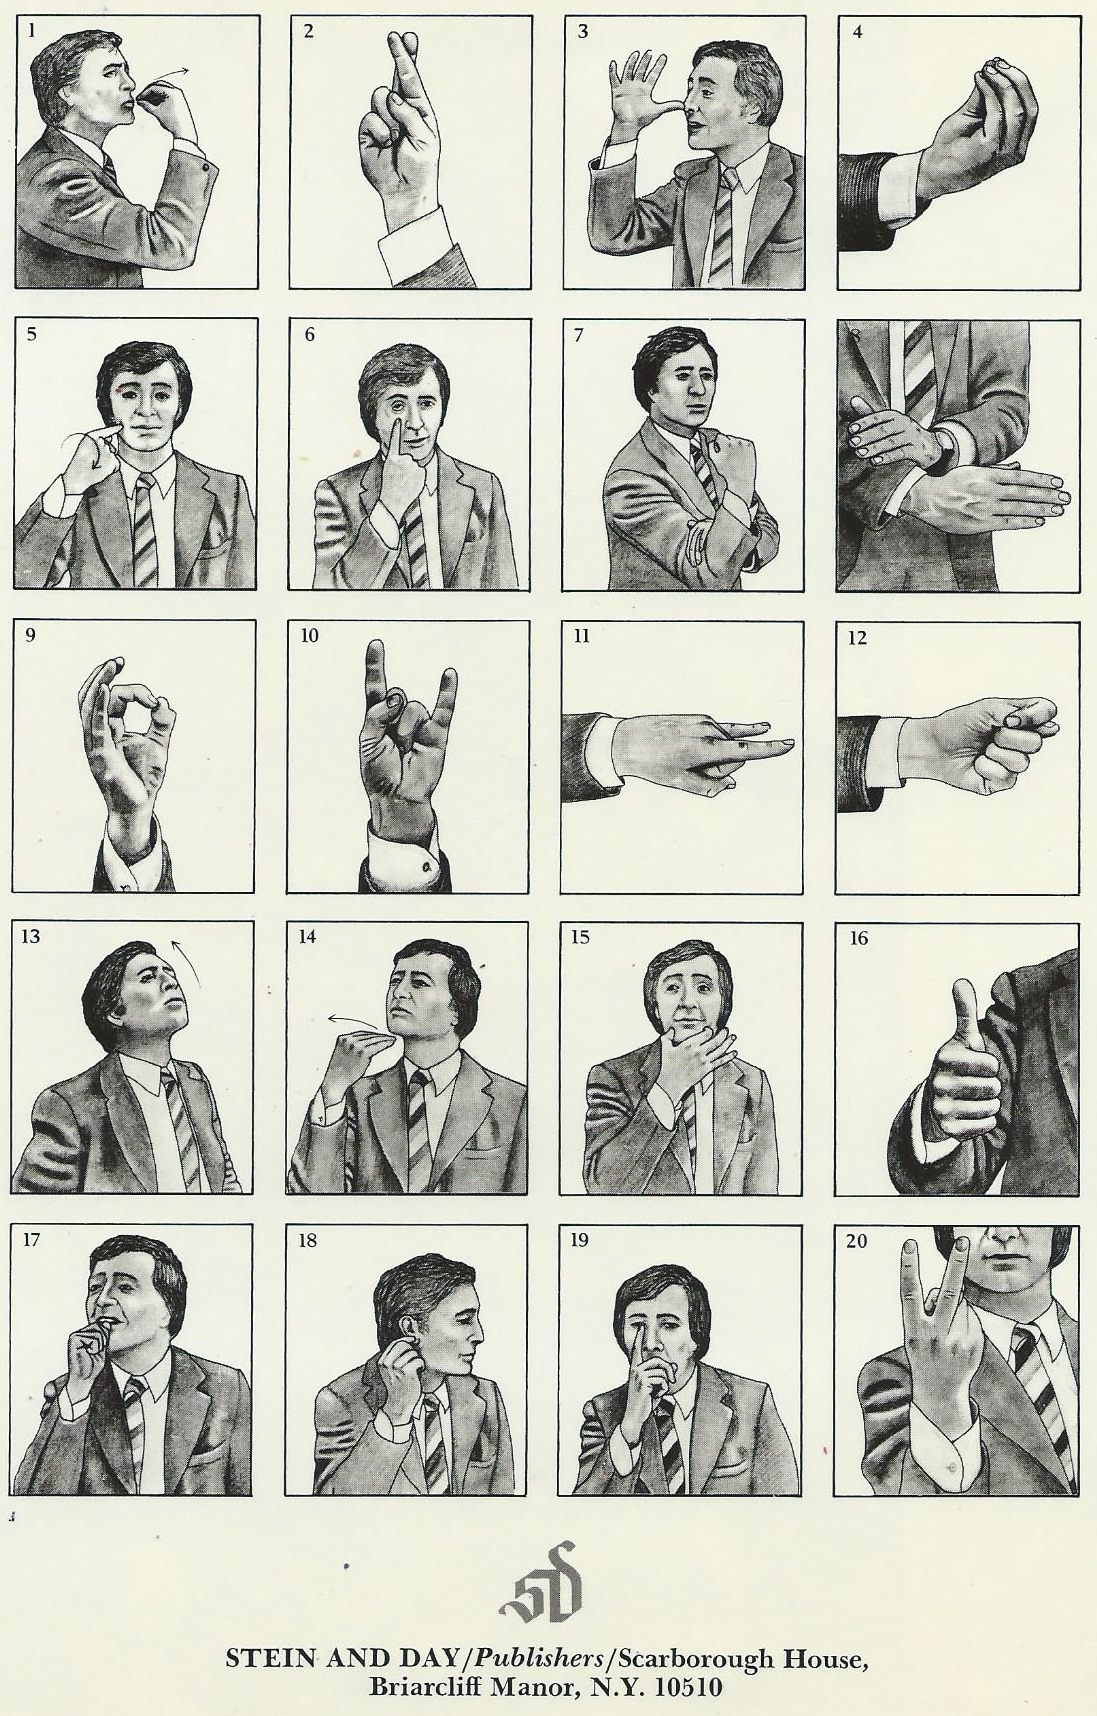
\includegraphics[width=0.80\textwidth]{figures/EmblemsMorris.png}
    \caption{\label{fig:Figure_Emblems_Morris}Representation of emblematic gestures}
\end{figure}
